\vspace{-10mm}
\section*{Part 2 [30 points]}

\begin{enumerate}
 
    \item \textbf{Interference behavior} \textbf{[19 points]}

    \begin{enumerate}

%%%%%%%%%%%%%%%%%%%%%%%%%%%%%%%%%%%%%%%%%%%
%%% QUESTION 2.1A

        \item \textbf{[11 points]} Fill in the following table with the normalized execution time of each batch job with each source of interference. The execution time should be normalized to the job’s execution time with no interference. Round the normalized execution time to 2 decimal places. Color-code each field in the table as follows: {\color{Green}\textbf{green}} if the normalized execution time is less than or equal to 1.3, {\color{YellowOrange}\textbf{orange}} if the normalized execution time is over 1.3 and up to 2, and {\color{Red}\textbf{red}} if the normalized execution time is greater than 2. Briefly summarize in a paragraph the resource interference sensitivity of each batch job. 

        % Fill in this table with your results
        \begin{center}
        \begin{tabular}{ |c|c|c|c|c|c|c|c| } 
        \hline
         \textbf{Workload} & \texttt{\textbf{none}} & \texttt{\textbf{cpu}} & \texttt{\textbf{l1d}} & \texttt{\textbf{l1i}} & \texttt{\textbf{l2}} & \texttt{\textbf{llc}} & \texttt{\textbf{memBW}}  \\
         \hline\hline
        blackscholes & 1.00 & \cellcolor{YellowOrange!75}1.31 & \cellcolor{Green!75}1.12 & \cellcolor{YellowOrange!75}1.54 & \cellcolor{Green!75}1.15 & \cellcolor{YellowOrange!75}1.49 & \cellcolor{YellowOrange!75}1.32 \\  \hline
        canneal & 1.00 & \cellcolor{Green!75}1.18 & \cellcolor{Green!75}1.21 & \cellcolor{YellowOrange!75}1.35 & \cellcolor{Green!75}1.18 & \cellcolor{YellowOrange!75}1.98 & \cellcolor{YellowOrange!75}1.31 \\  \hline
        dedup & 1.00 & \cellcolor{YellowOrange!75}1.66 & \cellcolor{Green!75}1.19 & \cellcolor{Red!75}2.04 & \cellcolor{Green!75}1.19 & \cellcolor{Red!75}2.19 & \cellcolor{YellowOrange!75}1.65 \\  \hline
        ferret & 1.00 & \cellcolor{YellowOrange!75}1.83 & \cellcolor{Green!75}1.00 & \cellcolor{Red!75}2.24 & \cellcolor{Green!75}1.01 & \cellcolor{Red!75}2.58 & \cellcolor{YellowOrange!75}1.93 \\  \hline
        freqmine & 1.00 & \cellcolor{Red!75}2.01 & \cellcolor{Green!75}1.02 & \cellcolor{Red!75}2.00 & \cellcolor{Green!75}1.04 & \cellcolor{YellowOrange!75}1.90 & \cellcolor{YellowOrange!75}1.61 \\  \hline
        radix & 1.00 & \cellcolor{Green!75}1.06 & \cellcolor{Green!75}1.07 & \cellcolor{Green!75}1.15 & \cellcolor{Green!75}1.05 & \cellcolor{YellowOrange!75}1.66 & \cellcolor{Green!75}1.10 \\  \hline
        vips & 1.00 & \cellcolor{YellowOrange!75}1.73 & \cellcolor{YellowOrange!75}1.60 & \cellcolor{YellowOrange!75}1.98 & \cellcolor{YellowOrange!75}1.60 & \cellcolor{Red!75}2.09 & \cellcolor{YellowOrange!75}1.76 \\  \hline
        \end{tabular}
        \end{center}
        
         % Here you place your brief summary.

         \textbf{Solution:} As can be seen in the table all jobs are affected by the \texttt{llc} interference. On the other hand,  \texttt{l1d} and \texttt{l2} are the tasks that interfere the least with the jobs. \texttt{memBW} also affect all of the jobs, but not in such a dramatic way as \texttt{llc}. \texttt{l1i} has also a high influence on execution time, more than \texttt{memBw}, although it is better than \texttt{llc} again, specially considering that \texttt{radix} is not very much affected by it. \texttt{cpu} can be considered slightly better than \texttt{l1i}.

         considering a more detail, per application, look we can notice that \textbf{vips} is the most resource demanding task as it is affected by all sources of interference. The least resource demanding tasks are \textbf{radix} and \textbf{canneal} this could imply that they are neither very CPU or data dependent. Nevertheless, some critical data should always be accessed and, as a consequence, the penalty of accessing memory after interference to \texttt{llc} is still noticeable. There are some similarities between \textbf{blackscholes}, \textbf{dedup}, \textbf{ferret}, and \textbf{freqmine} as they are all visibly CPU and data dependent with noticeable drops in performance, although the least affected one is \textbf{blackscholes}.
    
%%%%%%%%%%%%%%%%%%%%%%%%%%%%%%%%%%%%%%%%%%%
%%% QUESTION 2.1B

        \item \textbf{[8 points]} Explain what the interference profile table tells you about the resource requirements for each application. Which jobs (if any) seem like good candidates to collocate with memcached from Part 1, without violating the SLO of 2 ms P95 latency at 40K QPS?

        % Here you place your solution. l1i and cpu dependent
        \textbf{Solution:} Given the poor performance of the applications when facing interference in \texttt{llc} we can say that all of the tasks are data intensive. An overused \texttt{llc} would imply a cache miss and memory access which is very detrimental to execution time, much more than misses to the previous levels of cache. This last points is reflected in the table, given that \texttt{l1d} and \texttt{l2} interference do not make a big difference on execution time. 
        
        Additionally, we can see a clear correlation between \texttt{cpu} and \texttt{l1i}. Applications that are most affected by \texttt{cpu} intereference are also the most affected by \texttt{l1i} interference. This clearly indicates that this tasks are in general computational intensive as they require to load a large number of instructions from cache and are CPU intensive. Following this thread, \textbf{radix} and \textbf{canneal} are clearly not very much CPU or memory dependent as they are not strained by their interference.

        According to the graph: \textbf{ferret}, \textbf{dedup}, \textbf{freqmine} and \textbf{blackscholes} are in order the applications that are the most CPU and memory dependent.
        
        Regarding the second part of the question, \texttt{memchached} was shown to be affected most by \texttt{cpu} and \texttt{l1i} interferences. Consequently, in order to not violate the SLO of 2 ms P95 latency at 40K QPS it would be best to collocate it with tasks that are not as dependent on CPU, given that at 40K the latency is already affected by these intereferences. Thus, the most suitable application would be \textbf{radix}, followed closely by \textbf{canneal} because even if it is slightly affected by  \texttt{l1i} we can still see that it is int the lower range of the orange color-code compared to the other tasks. Last, if needed, it could also be possible to collocate it with \textbf{blacksholes} for the same reasons as \textbf{canneal}, but it should be the last option among theese three since it is slightly worse than \textbf{canneal}.
        
    \end{enumerate}
    
    \vspace{-2mm}
    \item \textbf{Parallel behavior} \textbf{[11 points]}

%%%%%%%%%%%%%%%%%%%%%%%%%%%%%%%%%%%%%%%%%%%
%%% QUESTION 2.2
    
    Plot a single line graph with speedup as the y-axis (normalized time to the single thread config,
    $\textrm{Time}_1$ / $\textrm{Time}_n)$ vs. number of threads on the x-axis (1, 2, 4 and 8 threads, see the project description for more details). Briefly discuss the scalability of each application: e.g.,
    linear/sub-linear/super-linear. Do the applications gain significant speedup with the increased number of threads? Explain what you consider to
    be ``significant''. 

    \begin{figure}[!h]
    \centering
    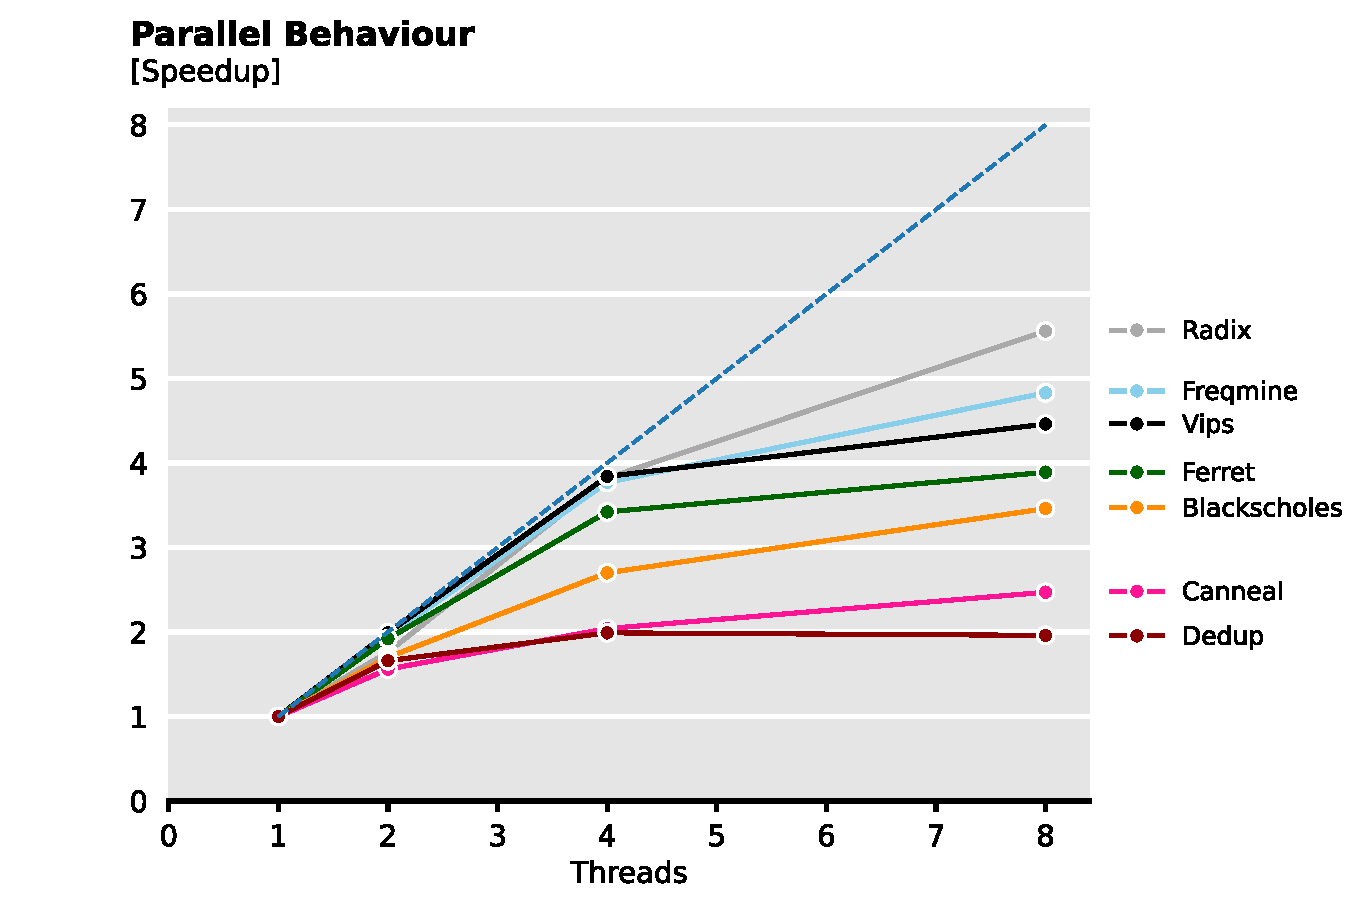
\includegraphics[width=0.76\textwidth]{figures/plot2b.pdf}
    \caption{\label{fig:plot1} Parallelization trends}
    \end{figure}

    % Here you place your solution.
    \textbf{Solution: }While all of the speedups are sublinear we can still notice some interesting facts. \textbf{canneal} and \textbf{dedup} are the tasks that benefit the least of the parallelization. While their speedup is significantly good with 4 threads as we obtained a 2 fold improvement, it is clearly not worth to add more threads as the performance stays the same or even gets slightly worse. This is probably due to the overhead of running and creating new threads. On the other hand, tasks \textbf{radix}, \textbf{freqmine} and \textbf{vips} are the most benefited in that order. Their paralellization offers diminishing returns as is expected by Amdahl's law, but it is still worth it to run 8 threads. Up to 4 threads the trend is almost linear, the slight difference is again probably due to the overhead of creating and running new threads. This graphical analysis can, therefore, help us figure out which applications are highly parallelizable and which are not allowing us to better distribute resources. 
    
\end{enumerate}

\newpage
